% Options for packages loaded elsewhere
\PassOptionsToPackage{unicode}{hyperref}
\PassOptionsToPackage{hyphens}{url}
\PassOptionsToPackage{dvipsnames,svgnames,x11names}{xcolor}
%
\documentclass[
]{article}
\usepackage{amsmath,amssymb}
\usepackage{iftex}
\ifPDFTeX
  \usepackage[T1]{fontenc}
  \usepackage[utf8]{inputenc}
  \usepackage{textcomp} % provide euro and other symbols
\else % if luatex or xetex
  \usepackage{unicode-math} % this also loads fontspec
  \defaultfontfeatures{Scale=MatchLowercase}
  \defaultfontfeatures[\rmfamily]{Ligatures=TeX,Scale=1}
\fi
\usepackage{lmodern}
\ifPDFTeX\else
  % xetex/luatex font selection
\fi
% Use upquote if available, for straight quotes in verbatim environments
\IfFileExists{upquote.sty}{\usepackage{upquote}}{}
\IfFileExists{microtype.sty}{% use microtype if available
  \usepackage[]{microtype}
  \UseMicrotypeSet[protrusion]{basicmath} % disable protrusion for tt fonts
}{}
\makeatletter
\@ifundefined{KOMAClassName}{% if non-KOMA class
  \IfFileExists{parskip.sty}{%
    \usepackage{parskip}
  }{% else
    \setlength{\parindent}{0pt}
    \setlength{\parskip}{6pt plus 2pt minus 1pt}}
}{% if KOMA class
  \KOMAoptions{parskip=half}}
\makeatother
\usepackage{xcolor}
\usepackage[margin=1in]{geometry}
\usepackage{color}
\usepackage{fancyvrb}
\newcommand{\VerbBar}{|}
\newcommand{\VERB}{\Verb[commandchars=\\\{\}]}
\DefineVerbatimEnvironment{Highlighting}{Verbatim}{commandchars=\\\{\}}
% Add ',fontsize=\small' for more characters per line
\usepackage{framed}
\definecolor{shadecolor}{RGB}{248,248,248}
\newenvironment{Shaded}{\begin{snugshade}}{\end{snugshade}}
\newcommand{\AlertTok}[1]{\textcolor[rgb]{0.94,0.16,0.16}{#1}}
\newcommand{\AnnotationTok}[1]{\textcolor[rgb]{0.56,0.35,0.01}{\textbf{\textit{#1}}}}
\newcommand{\AttributeTok}[1]{\textcolor[rgb]{0.13,0.29,0.53}{#1}}
\newcommand{\BaseNTok}[1]{\textcolor[rgb]{0.00,0.00,0.81}{#1}}
\newcommand{\BuiltInTok}[1]{#1}
\newcommand{\CharTok}[1]{\textcolor[rgb]{0.31,0.60,0.02}{#1}}
\newcommand{\CommentTok}[1]{\textcolor[rgb]{0.56,0.35,0.01}{\textit{#1}}}
\newcommand{\CommentVarTok}[1]{\textcolor[rgb]{0.56,0.35,0.01}{\textbf{\textit{#1}}}}
\newcommand{\ConstantTok}[1]{\textcolor[rgb]{0.56,0.35,0.01}{#1}}
\newcommand{\ControlFlowTok}[1]{\textcolor[rgb]{0.13,0.29,0.53}{\textbf{#1}}}
\newcommand{\DataTypeTok}[1]{\textcolor[rgb]{0.13,0.29,0.53}{#1}}
\newcommand{\DecValTok}[1]{\textcolor[rgb]{0.00,0.00,0.81}{#1}}
\newcommand{\DocumentationTok}[1]{\textcolor[rgb]{0.56,0.35,0.01}{\textbf{\textit{#1}}}}
\newcommand{\ErrorTok}[1]{\textcolor[rgb]{0.64,0.00,0.00}{\textbf{#1}}}
\newcommand{\ExtensionTok}[1]{#1}
\newcommand{\FloatTok}[1]{\textcolor[rgb]{0.00,0.00,0.81}{#1}}
\newcommand{\FunctionTok}[1]{\textcolor[rgb]{0.13,0.29,0.53}{\textbf{#1}}}
\newcommand{\ImportTok}[1]{#1}
\newcommand{\InformationTok}[1]{\textcolor[rgb]{0.56,0.35,0.01}{\textbf{\textit{#1}}}}
\newcommand{\KeywordTok}[1]{\textcolor[rgb]{0.13,0.29,0.53}{\textbf{#1}}}
\newcommand{\NormalTok}[1]{#1}
\newcommand{\OperatorTok}[1]{\textcolor[rgb]{0.81,0.36,0.00}{\textbf{#1}}}
\newcommand{\OtherTok}[1]{\textcolor[rgb]{0.56,0.35,0.01}{#1}}
\newcommand{\PreprocessorTok}[1]{\textcolor[rgb]{0.56,0.35,0.01}{\textit{#1}}}
\newcommand{\RegionMarkerTok}[1]{#1}
\newcommand{\SpecialCharTok}[1]{\textcolor[rgb]{0.81,0.36,0.00}{\textbf{#1}}}
\newcommand{\SpecialStringTok}[1]{\textcolor[rgb]{0.31,0.60,0.02}{#1}}
\newcommand{\StringTok}[1]{\textcolor[rgb]{0.31,0.60,0.02}{#1}}
\newcommand{\VariableTok}[1]{\textcolor[rgb]{0.00,0.00,0.00}{#1}}
\newcommand{\VerbatimStringTok}[1]{\textcolor[rgb]{0.31,0.60,0.02}{#1}}
\newcommand{\WarningTok}[1]{\textcolor[rgb]{0.56,0.35,0.01}{\textbf{\textit{#1}}}}
\usepackage{graphicx}
\makeatletter
\def\maxwidth{\ifdim\Gin@nat@width>\linewidth\linewidth\else\Gin@nat@width\fi}
\def\maxheight{\ifdim\Gin@nat@height>\textheight\textheight\else\Gin@nat@height\fi}
\makeatother
% Scale images if necessary, so that they will not overflow the page
% margins by default, and it is still possible to overwrite the defaults
% using explicit options in \includegraphics[width, height, ...]{}
\setkeys{Gin}{width=\maxwidth,height=\maxheight,keepaspectratio}
% Set default figure placement to htbp
\makeatletter
\def\fps@figure{htbp}
\makeatother
\setlength{\emergencystretch}{3em} % prevent overfull lines
\providecommand{\tightlist}{%
  \setlength{\itemsep}{0pt}\setlength{\parskip}{0pt}}
\setcounter{secnumdepth}{5}
\usepackage[french]{babel}
\ifLuaTeX
  \usepackage{selnolig}  % disable illegal ligatures
\fi
\usepackage{bookmark}
\IfFileExists{xurl.sty}{\usepackage{xurl}}{} % add URL line breaks if available
\urlstyle{same}
\hypersetup{
  pdfauthor={Manal Derghal, Khalil Ounis, Taqwa Ben Romdhane},
  colorlinks=true,
  linkcolor={Maroon},
  filecolor={Maroon},
  citecolor={Blue},
  urlcolor={blue},
  pdfcreator={LaTeX via pandoc}}

\title{Analyse des algorithmes de Maximum Subarray 1D\\
\strut ~M2 Data Science Algorithmique}
\author{Manal Derghal, Khalil Ounis, Taqwa Ben Romdhane}
\date{Lundi 7 avril 2025}

\begin{document}
\maketitle

{
\hypersetup{linkcolor=}
\setcounter{tocdepth}{2}
\tableofcontents
}
\noindent\hrulefill

\section{Description du problème et
objectif}\label{description-du-probluxe8me-et-objectif}

Le problème du Maximum Subarray 1D consiste à trouver la sous-séquence
contiguë d'un tableau numérique dont la somme des éléments est maximale.
Ce problème classique en algorithmique a des applications en analyse de
données financières, bioinformatique et traitement du signal.

\href{https://en.wikipedia.org/wiki/Maximum_subarray_problem}{La page
Wikipedia du Maximum Subarray} présente plusieurs approches
algorithmiques pour résoudre ce problème. Nous nous concentrons sur deux
méthodes :

\begin{enumerate}
\def\labelenumi{\arabic{enumi}.}
\tightlist
\item
  Algorithme naïf : complexité O(n²)
\item
  Algorithme de Kadane : complexité optimale O(n)
\end{enumerate}

Nos objectifs sont :\\
a. d'implémenter ces algorithmes en R et C++ et évaluer le gain de
temps.\\
b. de confirmer les complexités théoriques par des simulations
intensives.

\begin{center}\rule{0.5\linewidth}{0.5pt}\end{center}

\section{Un premier exemple}\label{un-premier-exemple}

Le package se télécharge ainsi :

\begin{Shaded}
\begin{Highlighting}[]
\NormalTok{devtools}\SpecialCharTok{::}\FunctionTok{install\_github}\NormalTok{(}\StringTok{"AMATERASU11/MaximumSubarray"}\NormalTok{)}
\end{Highlighting}
\end{Shaded}

et ses fonctions sont rendues disponibles sur Rstudio ainsi :

\begin{Shaded}
\begin{Highlighting}[]
\FunctionTok{library}\NormalTok{(MaximumSubarray)}
\end{Highlighting}
\end{Shaded}

On simule un petit exemple d'un vecteur \texttt{v} de taille
\texttt{100}

\begin{Shaded}
\begin{Highlighting}[]
\FunctionTok{set.seed}\NormalTok{(}\DecValTok{123}\NormalTok{)}
\NormalTok{v }\OtherTok{\textless{}{-}} \FunctionTok{sample}\NormalTok{(}\SpecialCharTok{{-}}\DecValTok{100}\SpecialCharTok{:}\DecValTok{100}\NormalTok{, }\DecValTok{100}\NormalTok{, }\AttributeTok{replace =} \ConstantTok{TRUE}\NormalTok{)}
\end{Highlighting}
\end{Shaded}

On teste les 4 algorithmes implémentés avec des noms explicites :

\begin{itemize}
\tightlist
\item
  \texttt{max\_subarray\_sum\_naive}
\item
  \texttt{max\_subarray\_sum\_opt}
\item
  \texttt{max\_subarray\_sum\_naive\_Rcpp}
\item
  \texttt{max\_subarray\_sum\_opt\_Rcpp}
\end{itemize}

Cela donne :

\begin{Shaded}
\begin{Highlighting}[]
\NormalTok{v}
\end{Highlighting}
\end{Shaded}

\begin{verbatim}
##   [1]  58  78 -87  94  69 -51  17 -58 -87  17  52 -11 -10  96 -10  84  -9  36
##  [19]  -2 -29 -75 -94  69  36  63 -23 -20 -58   2  16 -25  42 -69   8 -94  36
##  [37]  68 -27 -78  54  87 -48  34 -48  54  65 -67 -32 -29 -25 -38  40  -4 -10
##  [55]  52 -63 -80 -60  74 -11 -41 -85  15  -7 -95  99 -15 -15 -62  58  17 -51
##  [73] -67 -97 -88 -32  26  52 -49 -79 -12  59 -76 -66  67  11 -71  39  58  20
##  [91]   9  57 -37  41  98 -34  50  21 -22 -16
\end{verbatim}

\begin{Shaded}
\begin{Highlighting}[]
\FunctionTok{max\_subarray\_sum\_naive}\NormalTok{(v)}
\end{Highlighting}
\end{Shaded}

\begin{verbatim}
## $sum
## [1] 329
## 
## $subarray
##  [1]  67  11 -71  39  58  20   9  57 -37  41  98 -34  50  21
\end{verbatim}

\begin{Shaded}
\begin{Highlighting}[]
\FunctionTok{max\_subarray\_sum\_naive\_Rcpp}\NormalTok{(v)}
\end{Highlighting}
\end{Shaded}

\begin{verbatim}
## $sum
## [1] 329
## 
## $subarray
##  [1]  67  11 -71  39  58  20   9  57 -37  41  98 -34  50  21
\end{verbatim}

\begin{Shaded}
\begin{Highlighting}[]
\FunctionTok{max\_subarray\_sum\_opt}\NormalTok{(v)}
\end{Highlighting}
\end{Shaded}

\begin{verbatim}
## $sum
## [1] 329
## 
## $subarray
##  [1]  67  11 -71  39  58  20   9  57 -37  41  98 -34  50  21
\end{verbatim}

\begin{Shaded}
\begin{Highlighting}[]
\FunctionTok{max\_subarray\_sum\_opt\_Rcpp}\NormalTok{(v)}
\end{Highlighting}
\end{Shaded}

\begin{verbatim}
## $sum
## [1] 329
## 
## $subarray
##  [1]  67  11 -71  39  58  20   9  57 -37  41  98 -34  50  21
\end{verbatim}

\begin{center}\rule{0.5\linewidth}{0.5pt}\end{center}

\section{Comparaison R avec C++}\label{comparaison-r-avec-c}

On va faire des comparaisons pour les deux types d'algorithme en R et
C++ pour quantifier leur différence de performance.

La fonction \texttt{one.simu.time} retourne le temps recherché, et
\texttt{one.simu} sera utilisé par \texttt{microbenchmark}, on retourne
le temps en ms

\begin{Shaded}
\begin{Highlighting}[]
\FunctionTok{library}\NormalTok{(microbenchmark)}

\NormalTok{one.simu.time }\OtherTok{\textless{}{-}} \ControlFlowTok{function}\NormalTok{(n, func) \{}
  
\NormalTok{  v }\OtherTok{\textless{}{-}} \FunctionTok{sample}\NormalTok{(}\SpecialCharTok{{-}}\DecValTok{100}\SpecialCharTok{:}\DecValTok{100}\NormalTok{, n, }\AttributeTok{replace =} \ConstantTok{TRUE}\NormalTok{)}

  \ControlFlowTok{if}\NormalTok{ (func }\SpecialCharTok{==} \StringTok{"Naive1D"}\NormalTok{) \{}
\NormalTok{    t }\OtherTok{\textless{}{-}} \FunctionTok{microbenchmark}\NormalTok{(}\FunctionTok{max\_subarray\_sum\_naive}\NormalTok{(v), }\AttributeTok{times =} \DecValTok{1}\NormalTok{)}\SpecialCharTok{$}\NormalTok{time }\SpecialCharTok{/} \FloatTok{1e6}
\NormalTok{  \} }\ControlFlowTok{else} \ControlFlowTok{if}\NormalTok{ (func }\SpecialCharTok{==} \StringTok{"Naive1D\_cpp"}\NormalTok{) \{}
\NormalTok{    t }\OtherTok{\textless{}{-}} \FunctionTok{microbenchmark}\NormalTok{(}\FunctionTok{max\_subarray\_sum\_naive\_Rcpp}\NormalTok{(v), }\AttributeTok{times =} \DecValTok{1}\NormalTok{)}\SpecialCharTok{$}\NormalTok{time }\SpecialCharTok{/} \FloatTok{1e6}
\NormalTok{  \} }\ControlFlowTok{else} \ControlFlowTok{if}\NormalTok{ (func }\SpecialCharTok{==} \StringTok{"Kadane1D"}\NormalTok{) \{}
\NormalTok{    t }\OtherTok{\textless{}{-}} \FunctionTok{microbenchmark}\NormalTok{(}\FunctionTok{max\_subarray\_sum\_opt}\NormalTok{(v), }\AttributeTok{times =} \DecValTok{1}\NormalTok{)}\SpecialCharTok{$}\NormalTok{time }\SpecialCharTok{/} \FloatTok{1e6}
\NormalTok{  \} }\ControlFlowTok{else} \ControlFlowTok{if}\NormalTok{ (func }\SpecialCharTok{==} \StringTok{"Kadane1D\_cpp"}\NormalTok{) \{}
\NormalTok{    t }\OtherTok{\textless{}{-}} \FunctionTok{microbenchmark}\NormalTok{(}\FunctionTok{max\_subarray\_sum\_opt\_Rcpp}\NormalTok{(v), }\AttributeTok{times =} \DecValTok{1}\NormalTok{)}\SpecialCharTok{$}\NormalTok{time }\SpecialCharTok{/} \FloatTok{1e6}
\NormalTok{  \} }\ControlFlowTok{else}\NormalTok{ \{}
    \FunctionTok{stop}\NormalTok{(}\StringTok{"fonction inconnue"}\NormalTok{)}
\NormalTok{  \}}

  \FunctionTok{return}\NormalTok{(}\FunctionTok{round}\NormalTok{(t, }\DecValTok{2}\NormalTok{))}
\NormalTok{\}}
\end{Highlighting}
\end{Shaded}

\subsection{Un essai}\label{un-essai}

\subsubsection{Temps d'exécution en R}\label{temps-dexuxe9cution-en-r}

Sur un exemple, on obtient :

\begin{Shaded}
\begin{Highlighting}[]
\CommentTok{\# Simulation sur une matrice de taille n}
\NormalTok{n }\OtherTok{\textless{}{-}} \DecValTok{10000}

\CommentTok{\# Exécuter la simulation}
\NormalTok{res\_naive }\OtherTok{\textless{}{-}} \FunctionTok{one.simu.time}\NormalTok{(n,}\StringTok{"Naive1D"}\NormalTok{)}
\NormalTok{res\_kadane }\OtherTok{\textless{}{-}} \FunctionTok{one.simu.time}\NormalTok{(n, }\StringTok{"Kadane1D"}\NormalTok{)}

\CommentTok{\# Afficher les résultats}
\FunctionTok{cat}\NormalTok{(}\StringTok{"time\_naive:"}\NormalTok{, res\_naive,}\StringTok{"ms}\SpecialCharTok{\textbackslash{}n}\StringTok{"}\NormalTok{)}
\end{Highlighting}
\end{Shaded}

\begin{verbatim}
## time_naive: 2167.17 ms
\end{verbatim}

\begin{Shaded}
\begin{Highlighting}[]
\FunctionTok{cat}\NormalTok{(}\StringTok{"time\_kadane:"}\NormalTok{, res\_kadane, }\StringTok{"ms"}\NormalTok{)}
\end{Highlighting}
\end{Shaded}

\begin{verbatim}
## time_kadane: 0.89 ms
\end{verbatim}

\subsubsection{Temps d'exécution en C++}\label{temps-dexuxe9cution-en-c}

sur une matrice de taille 30x50, on obtient les résultats suivants :

\begin{Shaded}
\begin{Highlighting}[]
\CommentTok{\# Simulation sur une matrice de taille n}
\NormalTok{n }\OtherTok{\textless{}{-}} \DecValTok{10000}

\NormalTok{res\_naive\_cpp }\OtherTok{\textless{}{-}} \FunctionTok{one.simu.time}\NormalTok{(n,}\StringTok{"Naive1D\_cpp"}\NormalTok{)}
\NormalTok{res\_Kadane\_cpp }\OtherTok{\textless{}{-}} \FunctionTok{one.simu.time}\NormalTok{(n,}\StringTok{"Kadane1D\_cpp"}\NormalTok{)}

\CommentTok{\# Afficher les résultats}
\FunctionTok{cat}\NormalTok{(}\StringTok{"time\_naive\_cpp:"}\NormalTok{ ,res\_naive\_cpp,}\StringTok{"ms}\SpecialCharTok{\textbackslash{}n}\StringTok{"}\NormalTok{)}
\end{Highlighting}
\end{Shaded}

\begin{verbatim}
## time_naive_cpp: 24.98 ms
\end{verbatim}

\begin{Shaded}
\begin{Highlighting}[]
\FunctionTok{cat}\NormalTok{(}\StringTok{"time\_kadane\_cpp:"}\NormalTok{,res\_Kadane\_cpp, }\StringTok{"ms"}\NormalTok{)}
\end{Highlighting}
\end{Shaded}

\begin{verbatim}
## time_kadane_cpp: 0.07 ms
\end{verbatim}

\subsection{Simulations avec
répétitions}\label{simulations-avec-ruxe9puxe9titions}

On reproduit ces comparaisons de manière plus robuste:

\begin{Shaded}
\begin{Highlighting}[]
\NormalTok{nbSimus }\OtherTok{\textless{}{-}} \DecValTok{10}

\NormalTok{time\_naive }\OtherTok{\textless{}{-}} \FunctionTok{rep}\NormalTok{(}\DecValTok{0}\NormalTok{, nbSimus); time\_naive\_cpp }\OtherTok{\textless{}{-}} \FunctionTok{rep}\NormalTok{(}\DecValTok{0}\NormalTok{, nbSimus);}
\NormalTok{time\_kadane }\OtherTok{\textless{}{-}} \FunctionTok{rep}\NormalTok{(}\DecValTok{0}\NormalTok{, nbSimus); time\_kadane\_cpp }\OtherTok{\textless{}{-}} \FunctionTok{rep}\NormalTok{(}\DecValTok{0}\NormalTok{, nbSimus)}

\ControlFlowTok{for}\NormalTok{(i }\ControlFlowTok{in} \DecValTok{1}\SpecialCharTok{:}\NormalTok{nbSimus)\{time\_naive[i] }\OtherTok{\textless{}{-}} \FunctionTok{one.simu.time}\NormalTok{(n, }\AttributeTok{func =} \StringTok{"Naive1D"}\NormalTok{)\}}
\ControlFlowTok{for}\NormalTok{(i }\ControlFlowTok{in} \DecValTok{1}\SpecialCharTok{:}\NormalTok{nbSimus)\{time\_naive\_cpp[i] }\OtherTok{\textless{}{-}} \FunctionTok{one.simu.time}\NormalTok{(n, }\AttributeTok{func =} \StringTok{"Naive1D\_cpp"}\NormalTok{)\}}
\ControlFlowTok{for}\NormalTok{(i }\ControlFlowTok{in} \DecValTok{1}\SpecialCharTok{:}\NormalTok{nbSimus)\{time\_kadane[i] }\OtherTok{\textless{}{-}} \FunctionTok{one.simu.time}\NormalTok{(n, }\AttributeTok{func =} \StringTok{"Kadane1D"}\NormalTok{)\}}
\ControlFlowTok{for}\NormalTok{(i }\ControlFlowTok{in} \DecValTok{1}\SpecialCharTok{:}\NormalTok{nbSimus)\{time\_kadane\_cpp[i] }\OtherTok{\textless{}{-}} \FunctionTok{one.simu.time}\NormalTok{(n, }\AttributeTok{func =} \StringTok{"Kadane1D\_cpp"}\NormalTok{)\}}
\end{Highlighting}
\end{Shaded}

\subsubsection{Gain R versus C++}\label{gain-r-versus-c}

\begin{Shaded}
\begin{Highlighting}[]
\NormalTok{naive\_speedup\_cpp }\OtherTok{\textless{}{-}} \FunctionTok{mean}\NormalTok{(time\_naive) }\SpecialCharTok{/} \FunctionTok{mean}\NormalTok{(time\_naive\_cpp)}
\NormalTok{kadane\_speedup\_cpp }\OtherTok{\textless{}{-}} \FunctionTok{mean}\NormalTok{(time\_kadane) }\SpecialCharTok{/} \FunctionTok{mean}\NormalTok{(time\_kadane\_cpp)}
\FunctionTok{cat}\NormalTok{(}\StringTok{"le gain R vs cpp pour naif:"}\NormalTok{, }\FunctionTok{round}\NormalTok{(naive\_speedup\_cpp,}\DecValTok{2}\NormalTok{),}\StringTok{"ms}\SpecialCharTok{\textbackslash{}n}\StringTok{"}\NormalTok{)}
\end{Highlighting}
\end{Shaded}

\begin{verbatim}
## le gain R vs cpp pour naif: 71.46 ms
\end{verbatim}

\begin{Shaded}
\begin{Highlighting}[]
\FunctionTok{cat}\NormalTok{(}\StringTok{"le gain R vs cpp pour Kadane:"}\NormalTok{, }\FunctionTok{round}\NormalTok{(kadane\_speedup\_cpp,}\DecValTok{2}\NormalTok{),}\StringTok{"ms}\SpecialCharTok{\textbackslash{}n}\StringTok{"}\NormalTok{)}
\end{Highlighting}
\end{Shaded}

\begin{verbatim}
## le gain R vs cpp pour Kadane: 9.88 ms
\end{verbatim}

\subsubsection{Gain Naif Versus Kadane en R et
C++}\label{gain-naif-versus-kadane-en-r-et-c}

\begin{Shaded}
\begin{Highlighting}[]
\NormalTok{kadane\_vs\_naive\_R }\OtherTok{\textless{}{-}} \FunctionTok{mean}\NormalTok{(time\_naive) }\SpecialCharTok{/} \FunctionTok{mean}\NormalTok{(time\_kadane)}
\NormalTok{kadane\_vs\_naive\_Rcpp }\OtherTok{\textless{}{-}} \FunctionTok{mean}\NormalTok{(time\_naive\_cpp) }\SpecialCharTok{/} \FunctionTok{mean}\NormalTok{(time\_kadane\_cpp)}
\FunctionTok{cat}\NormalTok{(}\StringTok{"le gain naif vs Kadane en R est:"}\NormalTok{,}\FunctionTok{round}\NormalTok{(kadane\_vs\_naive\_R,}\DecValTok{2}\NormalTok{), }\StringTok{"ms}\SpecialCharTok{\textbackslash{}n}\StringTok{"}\NormalTok{)}
\end{Highlighting}
\end{Shaded}

\begin{verbatim}
## le gain naif vs Kadane en R est: 2030.39 ms
\end{verbatim}

\begin{Shaded}
\begin{Highlighting}[]
\FunctionTok{cat}\NormalTok{(}\StringTok{"le gain cpp est:"}\NormalTok{,}\FunctionTok{round}\NormalTok{(kadane\_vs\_naive\_Rcpp,}\DecValTok{2}\NormalTok{), }\StringTok{"ms}\SpecialCharTok{\textbackslash{}n}\StringTok{"}\NormalTok{)}
\end{Highlighting}
\end{Shaded}

\begin{verbatim}
## le gain cpp est: 280.81 ms
\end{verbatim}

On recommence avec \texttt{n\ =\ 20000} seulement pour le gain avec C++
pour Kadane

\begin{Shaded}
\begin{Highlighting}[]
\FunctionTok{set.seed}\NormalTok{(}\DecValTok{123}\NormalTok{)}
\NormalTok{n }\OtherTok{\textless{}{-}} \DecValTok{20000}
\NormalTok{nbSimus }\OtherTok{\textless{}{-}} \DecValTok{10}
\NormalTok{time\_kadane }\OtherTok{\textless{}{-}} \FunctionTok{rep}\NormalTok{(}\DecValTok{0}\NormalTok{, nbSimus); time\_kadane\_cpp }\OtherTok{\textless{}{-}} \FunctionTok{rep}\NormalTok{(}\DecValTok{0}\NormalTok{, nbSimus)}
\ControlFlowTok{for}\NormalTok{(i }\ControlFlowTok{in} \DecValTok{1}\SpecialCharTok{:}\NormalTok{nbSimus)\{time\_kadane[i] }\OtherTok{\textless{}{-}} \FunctionTok{one.simu.time}\NormalTok{(n, }\AttributeTok{func =} \StringTok{"Kadane1D"}\NormalTok{)\}}
\ControlFlowTok{for}\NormalTok{(i }\ControlFlowTok{in} \DecValTok{1}\SpecialCharTok{:}\NormalTok{nbSimus)\{time\_kadane\_cpp[i] }\OtherTok{\textless{}{-}} \FunctionTok{one.simu.time}\NormalTok{(n, }\AttributeTok{func =} \StringTok{"Kadane1D\_cpp"}\NormalTok{)\}}
\NormalTok{median\_kadane\_R\_vs\_Rcpp }\OtherTok{\textless{}{-}} \FunctionTok{median}\NormalTok{(time\_kadane) }\SpecialCharTok{/} \FunctionTok{median}\NormalTok{(time\_kadane\_cpp)}
\FunctionTok{cat}\NormalTok{(}\StringTok{"le gain Kadane en R vs Kadane en C++ est:"}\NormalTok{,}\FunctionTok{round}\NormalTok{(median\_kadane\_R\_vs\_Rcpp,}\DecValTok{2}\NormalTok{), }\StringTok{"ms}\SpecialCharTok{\textbackslash{}n}\StringTok{"}\NormalTok{)}
\end{Highlighting}
\end{Shaded}

\begin{verbatim}
## le gain Kadane en R vs Kadane en C++ est: 11.86 ms
\end{verbatim}

\textbf{Conclusion:}

\subsubsection{Performances C++ vs R :}\label{performances-c-vs-r}

\begin{itemize}
\tightlist
\item
  Naïf : C++ 71× plus rapide\\
\item
  Kadane : C++ 10× plus rapide → 12× pour n=20k
\end{itemize}

\subsubsection{Efficacité algorithmique
:}\label{efficacituxe9-algorithmique}

\begin{itemize}
\item
  Kadane 2030× mieux que naïf en R\\
\item
  Kadane 281× mieux que naïf en C++
\end{itemize}

\subsection{\texorpdfstring{Simulations avec
\texttt{microbenchmark}}{Simulations avec microbenchmark}}\label{simulations-avec-microbenchmark}

Vous avez besoin des packages \texttt{microbenchmark} et
\texttt{ggplot2} pour exécuter les simulations et afficher les résultats
(sous forme de diagrammes en violon). Nous comparons
\texttt{naive\_Rcpp} avec \texttt{opt\_Rcpp} pour des tailles de données
\texttt{n\ =\ 1000}, \texttt{n\ =\ 5000} et \texttt{n\ =\ 10000}.

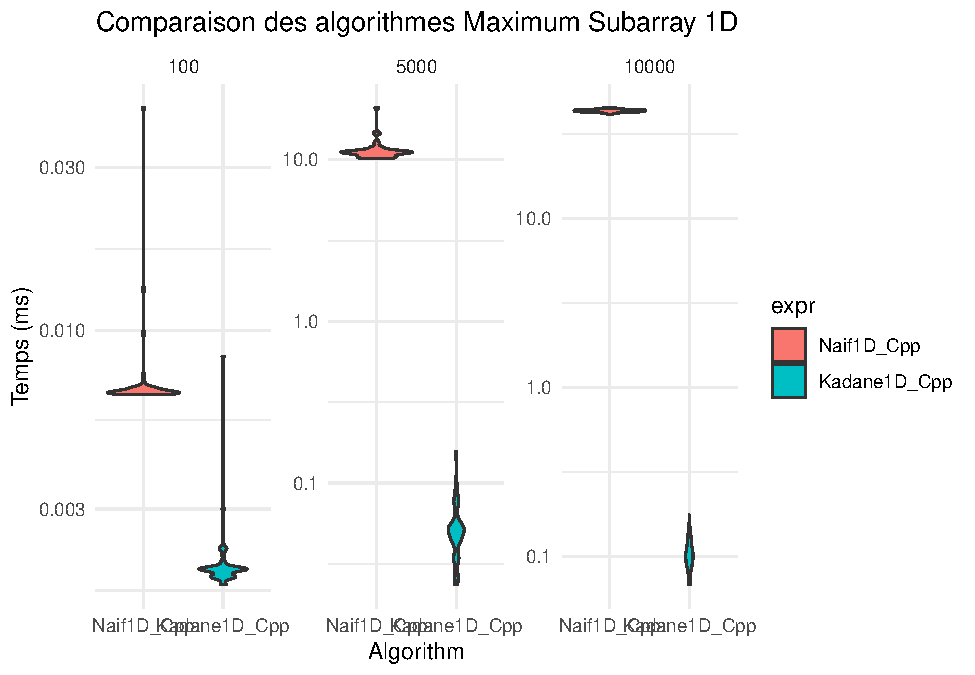
\includegraphics{MaxSubarray1D_files/figure-latex/benchmark-1.pdf}

\begin{verbatim}
## # A tibble: 6 x 8
##       n expr         min_time  q1_time median_time mean_time  q3_time max_time
##   <dbl> <fct>           <dbl>    <dbl>       <dbl>     <dbl>    <dbl>    <dbl>
## 1   100 Naif1D_Cpp    0.00650  0.00653     0.00660   0.00761  0.00678  0.0449 
## 2   100 Kadane1D_Cpp  0.00180  0.00190     0.00200   0.00214  0.00200  0.00840
## 3  5000 Naif1D_Cpp   10.2     10.7        11.1      11.4     11.4     20.9    
## 4  5000 Kadane1D_Cpp  0.0235   0.0432      0.0504    0.0527   0.0549   0.156  
## 5 10000 Naif1D_Cpp   41.3     42.8        43.2      43.2     43.7     45.0    
## 6 10000 Kadane1D_Cpp  0.0683   0.0910      0.102     0.104    0.114    0.176
\end{verbatim}

\begin{center}\rule{0.5\linewidth}{0.5pt}\end{center}

\section{Evaluation de la
complexité}\label{evaluation-de-la-complexituxe9}

Les vecteurs de longueurs \texttt{vector\_n\_naive} et
\texttt{vector\_n\_kadane} (\texttt{n} dans les dataframes) sont choisis
sur l'echelle logarithmique afin d'avoir un pas constant sur l'échelle
logarithmique en abscisse pour la régression.

On réalise 10 répétitions pour chaque valeur de \texttt{n} et pour
chaque algorithme. Les barres d'erreur sont placées en ``mean +/- sd''.

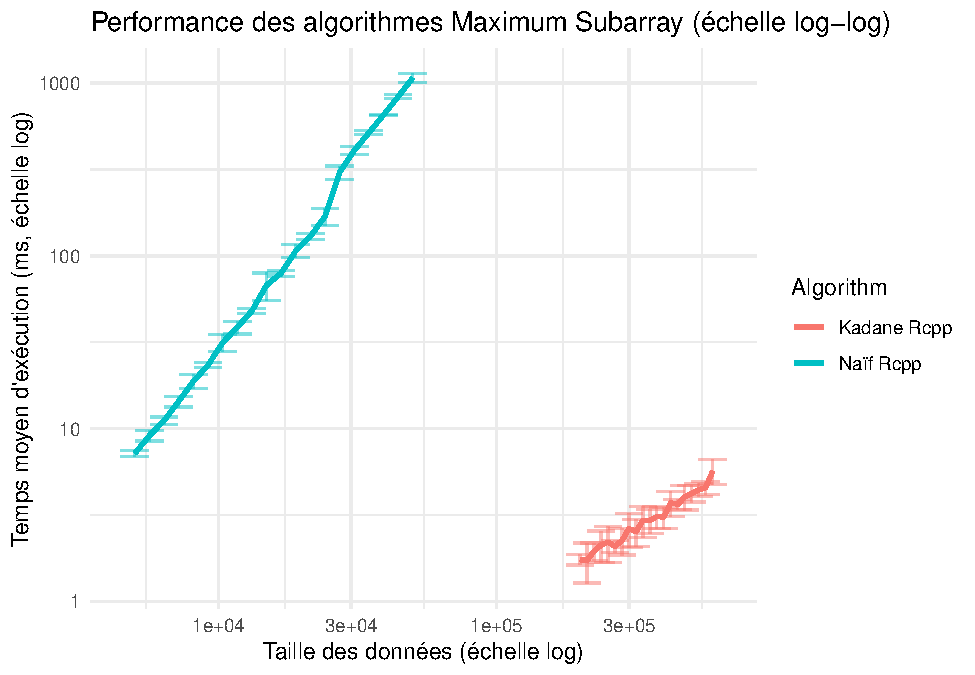
\includegraphics{MaxSubarray1D_files/figure-latex/simu complexite-1.pdf}

\begin{Shaded}
\begin{Highlighting}[]
\CommentTok{\# Affichage des résultats}
\FunctionTok{cat}\NormalTok{(}\StringTok{"Les résultats pour la solution naïve:}\SpecialCharTok{\textbackslash{}n}\StringTok{"}\NormalTok{)}
\end{Highlighting}
\end{Shaded}

\begin{verbatim}
## Les résultats pour la solution naïve:
\end{verbatim}

\begin{Shaded}
\begin{Highlighting}[]
\NormalTok{res\_Naive}
\end{Highlighting}
\end{Shaded}

\begin{verbatim}
##        n mean_time     sd_time
## 1   5000    11.270   0.5793291
## 2   5644    14.518   0.6674129
## 3   6371    18.123   0.3564345
## 4   7192    23.257   1.8599286
## 5   8119    30.168   1.8597539
## 6   9165    38.156   4.6008651
## 7  10346    47.265   0.7614496
## 8  11679    60.469   2.0857530
## 9  13183    75.990   2.2458455
## 10 14882    97.693   3.6680060
## 11 16799   130.050  18.9493694
## 12 18963   163.516  16.9388588
## 13 21407   198.468   3.3364112
## 14 24165   252.345   3.1644949
## 15 27278   321.789   4.4165206
## 16 30792   410.089   5.2821954
## 17 34760   520.307   3.1626292
## 18 39238   661.620  10.1094609
## 19 44293   638.637 205.7220376
## 20 50000   635.950 129.0299659
\end{verbatim}

\begin{Shaded}
\begin{Highlighting}[]
\FunctionTok{cat}\NormalTok{(}\StringTok{"Les résultats pour la solution optimale:}\SpecialCharTok{\textbackslash{}n}\StringTok{"}\NormalTok{)}
\end{Highlighting}
\end{Shaded}

\begin{verbatim}
## Les résultats pour la solution optimale:
\end{verbatim}

\begin{Shaded}
\begin{Highlighting}[]
\NormalTok{res\_Kadane}
\end{Highlighting}
\end{Shaded}

\begin{verbatim}
##         n mean_time    sd_time
## 1  100000     0.930 0.10392305
## 2  108840     0.998 0.06425643
## 3  118461     1.118 0.09807027
## 4  128933     1.296 0.21700998
## 5  140330     1.344 0.12790622
## 6  152735     1.448 0.09600926
## 7  166237     1.653 0.26268063
## 8  180932     1.704 0.26412118
## 9  196926     1.771 0.17175241
## 10 214334     2.010 0.18342422
## 11 233281     2.025 0.09454570
## 12 253902     2.236 0.15471838
## 13 276347     2.344 0.05541761
## 14 300776     2.660 0.16096929
## 15 327364     3.010 0.37151342
## 16 356302     3.049 0.13395273
## 17 387799     3.395 0.22979459
## 18 422079     3.648 0.18960778
## 19 459391     3.938 0.25827634
## 20 500000     4.532 0.52119094
\end{verbatim}

On vérifie la valeur du coefficient directeur pour les deux méthodes:

\begin{verbatim}
## 
## Call:
## lm(formula = log(res_Naive$mean_time) ~ log(res_Naive$n))
## 
## Residuals:
##      Min       1Q   Median       3Q      Max 
## -0.37749 -0.03897  0.00767  0.08380  0.11841 
## 
## Coefficients:
##                   Estimate Std. Error t value Pr(>|t|)    
## (Intercept)      -13.53834    0.35982  -37.62   <2e-16 ***
## log(res_Naive$n)   1.88275    0.03712   50.72   <2e-16 ***
## ---
## Signif. codes:  0 '***' 0.001 '**' 0.01 '*' 0.05 '.' 0.1 ' ' 1
## 
## Residual standard error: 0.116 on 18 degrees of freedom
## Multiple R-squared:  0.9931, Adjusted R-squared:  0.9927 
## F-statistic:  2573 on 1 and 18 DF,  p-value: < 2.2e-16
\end{verbatim}

\begin{verbatim}
## Exposant estimé (naïf): 1.882751
\end{verbatim}

\begin{verbatim}
## 
## Call:
## lm(formula = log(res_Kadane$mean_time) ~ log(res_Kadane$n))
## 
## Residuals:
##       Min        1Q    Median        3Q       Max 
## -0.056489 -0.026127 -0.008281  0.020889  0.067536 
## 
## Coefficients:
##                   Estimate Std. Error t value Pr(>|t|)    
## (Intercept)       -10.7594     0.2071  -51.95   <2e-16 ***
## log(res_Kadane$n)   0.9312     0.0168   55.43   <2e-16 ***
## ---
## Signif. codes:  0 '***' 0.001 '**' 0.01 '*' 0.05 '.' 0.1 ' ' 1
## 
## Residual standard error: 0.0367 on 18 degrees of freedom
## Multiple R-squared:  0.9942, Adjusted R-squared:  0.9939 
## F-statistic:  3073 on 1 and 18 DF,  p-value: < 2.2e-16
\end{verbatim}

\begin{verbatim}
## Exposant estimé (Kadane): 0.9312324
\end{verbatim}

Les coefficients directeurs trouvés sont bien ceux que l'on attendait.
La valeur 2 pour la méthode naïve et 1 pour l'algorithme de Kadane

\begin{center}\rule{0.5\linewidth}{0.5pt}\end{center}

\section{Cas particulier des données presques
triées}\label{cas-particulier-des-donnuxe9es-presques-triuxe9es}

On considère des données triées avec 5\% de valeurs échangées au hasard.

Sur un exemple cela donne :

\begin{Shaded}
\begin{Highlighting}[]
\NormalTok{v }\OtherTok{\textless{}{-}} \DecValTok{1}\SpecialCharTok{:}\DecValTok{100}
\NormalTok{n\_swap }\OtherTok{\textless{}{-}} \FunctionTok{floor}\NormalTok{(}\FloatTok{0.05} \SpecialCharTok{*} \FunctionTok{length}\NormalTok{(v))}
\NormalTok{swap\_indices }\OtherTok{\textless{}{-}} \FunctionTok{sample}\NormalTok{(}\FunctionTok{length}\NormalTok{(v), n\_swap)}
\NormalTok{v[swap\_indices] }\OtherTok{\textless{}{-}} \FunctionTok{sample}\NormalTok{(v[swap\_indices])}
\NormalTok{v}
\end{Highlighting}
\end{Shaded}

\begin{verbatim}
##   [1]   1   2   3   4   5   6   7   8   9  10  11  12  13  14  15  16  17  30
##  [19]  19  20  21  22  23  24  25  26  27  28  29  34  31  32  33  94  35  36
##  [37]  37  38  39  40  41  42  43  44  45  46  47  48  49  50  51  52  53  54
##  [55]  55  56  57  58  59  60  61  62  63  64  65  66  67  68  69  70  71  72
##  [73]  73  74  75  76  77  78  79  80  81  82  83  84  85  86  87  88  89  90
##  [91]  91  92  93  18  95  96  97  98  99 100
\end{verbatim}

\begin{Shaded}
\begin{Highlighting}[]
\CommentTok{\# Fonctions de simulation}
\NormalTok{one.simu }\OtherTok{\textless{}{-}} \ControlFlowTok{function}\NormalTok{(n, func) \{}
\NormalTok{  v }\OtherTok{\textless{}{-}} \FunctionTok{sample}\NormalTok{(}\SpecialCharTok{{-}}\DecValTok{100}\SpecialCharTok{:}\DecValTok{100}\NormalTok{, n, }\AttributeTok{replace =} \ConstantTok{TRUE}\NormalTok{)}
  \ControlFlowTok{if}\NormalTok{ (func }\SpecialCharTok{==} \StringTok{"naive\_Rcpp"}\NormalTok{) }\FunctionTok{return}\NormalTok{(}\FunctionTok{max\_subarray\_sum\_naive\_Rcpp}\NormalTok{(v))}
  \ControlFlowTok{if}\NormalTok{ (func }\SpecialCharTok{==} \StringTok{"kadane\_Rcpp"}\NormalTok{) }\FunctionTok{return}\NormalTok{(}\FunctionTok{max\_subarray\_sum\_opt\_Rcpp}\NormalTok{(v))}
\NormalTok{\}}

\NormalTok{one.simu2 }\OtherTok{\textless{}{-}} \ControlFlowTok{function}\NormalTok{(n, func) \{}
\NormalTok{  v }\OtherTok{\textless{}{-}} \DecValTok{1}\SpecialCharTok{:}\NormalTok{n}
\NormalTok{  n\_swap }\OtherTok{\textless{}{-}} \FunctionTok{floor}\NormalTok{(}\FloatTok{0.05} \SpecialCharTok{*}\NormalTok{ n)}
\NormalTok{  swap\_indices }\OtherTok{\textless{}{-}} \FunctionTok{sample}\NormalTok{(n, n\_swap)}
\NormalTok{  v[swap\_indices] }\OtherTok{\textless{}{-}} \FunctionTok{sample}\NormalTok{(v[swap\_indices])}
  \ControlFlowTok{if}\NormalTok{ (func }\SpecialCharTok{==} \StringTok{"naive\_Rcpp"}\NormalTok{) }\FunctionTok{return}\NormalTok{(}\FunctionTok{max\_subarray\_sum\_naive\_Rcpp}\NormalTok{(v))}
  \ControlFlowTok{if}\NormalTok{ (func }\SpecialCharTok{==} \StringTok{"kadane\_Rcpp"}\NormalTok{) }\FunctionTok{return}\NormalTok{(}\FunctionTok{max\_subarray\_sum\_opt\_Rcpp}\NormalTok{(v))}
\NormalTok{\}}
\end{Highlighting}
\end{Shaded}

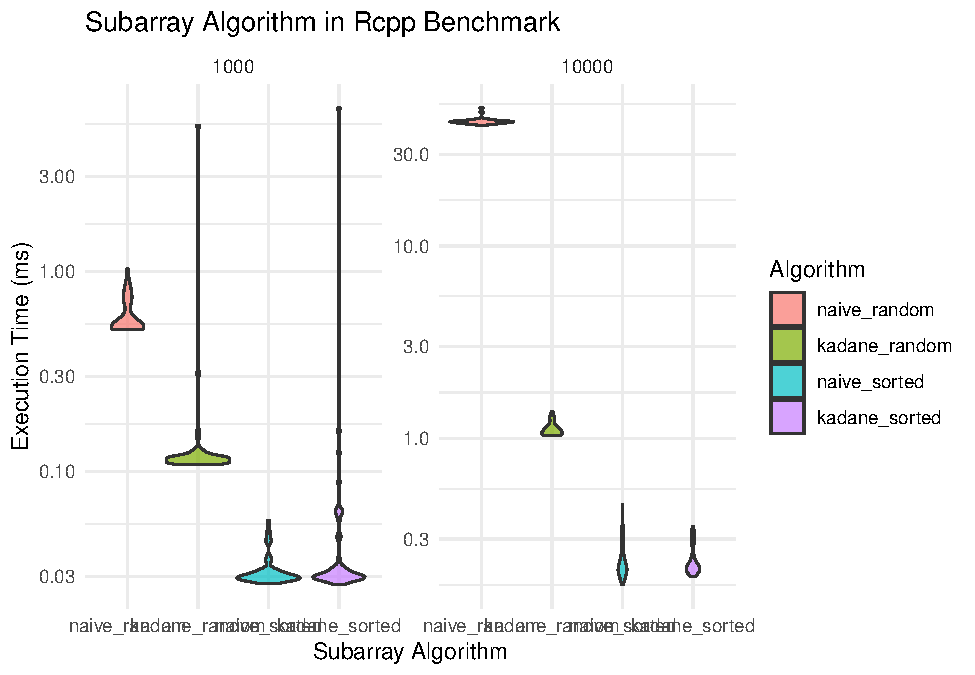
\includegraphics{MaxSubarray1D_files/figure-latex/benchmark2-1.pdf}

\begin{verbatim}
## # A tibble: 8 x 10
##       n expr       min_time q1_time median_time mean_time q3_time max_time type 
##   <dbl> <fct>         <dbl>   <dbl>       <dbl>     <dbl>   <dbl>    <dbl> <chr>
## 1  1000 naive_ran~   0.513   0.518       0.542     0.604   0.706    1.03   rand~
## 2  1000 kadane_ra~   0.109   0.111       0.116     0.226   0.120    5.38   rand~
## 3  1000 naive_sor~   0.0276  0.0290      0.0300    0.0321  0.0318   0.0567 sort~
## 4  1000 kadane_so~   0.0272  0.0295      0.0303    0.171   0.0331   6.59   sort~
## 5 10000 naive_ran~  42.5    43.7        44.3      44.4    44.7     52.2    rand~
## 6 10000 kadane_ra~   1.04    1.06        1.10      1.12    1.16     1.38   rand~
## 7 10000 naive_sor~   0.174   0.203       0.213     0.238   0.260    0.455  sort~
## 8 10000 kadane_so~   0.192   0.206       0.217     0.234   0.236    0.348  sort~
## # i 1 more variable: algo <chr>
\end{verbatim}

Pour n = 1000, le temps d'exécution est plus rapide que pour n = 10000.
Kadane est toujours plus rapide que Naïf, avec un écart plus important à
n = 10000. Lorsque les tableaux sont triés, Naïf et Kadane sont beaucoup
plus rapides, avec un écart réduit entre les deux.

\end{document}
